\documentclass[10pt]{beamer}
\usetheme{Malmoe}
\setbeamertemplate{navigation symbols}{}
%\colorlet{beamer@blendedblue}{blue!40!black}
\setbeamertemplate{navigation symbols}{}
\newcommand*\oldmacro{}%
\let\oldmacro\insertshorttitle%
\renewcommand*\insertshorttitle{%
\oldmacro\hfill%
\insertframenumber\,/\,\inserttotalframenumber}

\usepackage{caption}
\usepackage{hyperref}
\usepackage[makeroom]{cancel}
\usepackage{ amssymb }
\usepackage{appendixnumberbeamer}
%\usepackage{tikz-feynman}
\usepackage{graphicx}
\begin{document}

\title{Nationwide: Telematics Assessment Exercises}
\author[Barkeloo]{Jason Barkeloo}

%\titlegraphic{\includegraphics[width=4cm]{../ATLAS-Logo-Ref-RGB.png}\hspace*{2.75cm}~%
%   \includegraphics[width=4cm]{../uo_logo_green_on_white_2.jpg}
%}

%\date{April 26, 2018}
\frame{\titlepage}
\frame{\frametitle{Table of Contents}\tableofcontents[hidesubsections]}
\section{Part 1: GPS Data}

\subsection{Analysis}

\frame{\frametitle{}
\begin{itemize}
\item
\end{itemize}
}

\frame{\frametitle{}
\begin{itemize}
\item
\end{itemize}
\centering
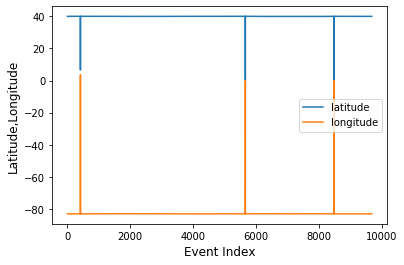
\includegraphics[width=0.7\textwidth]{Images/Image1.png}
}

\frame{\frametitle{}
\begin{itemize}
\item
\end{itemize}
\centering
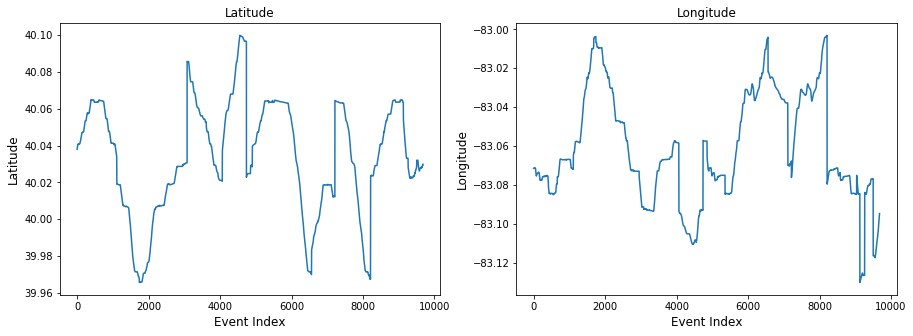
\includegraphics[width=1.\textwidth]{Images/Image2.png}
}

\frame{\frametitle{}
\begin{itemize}
\item
\end{itemize}
\centering
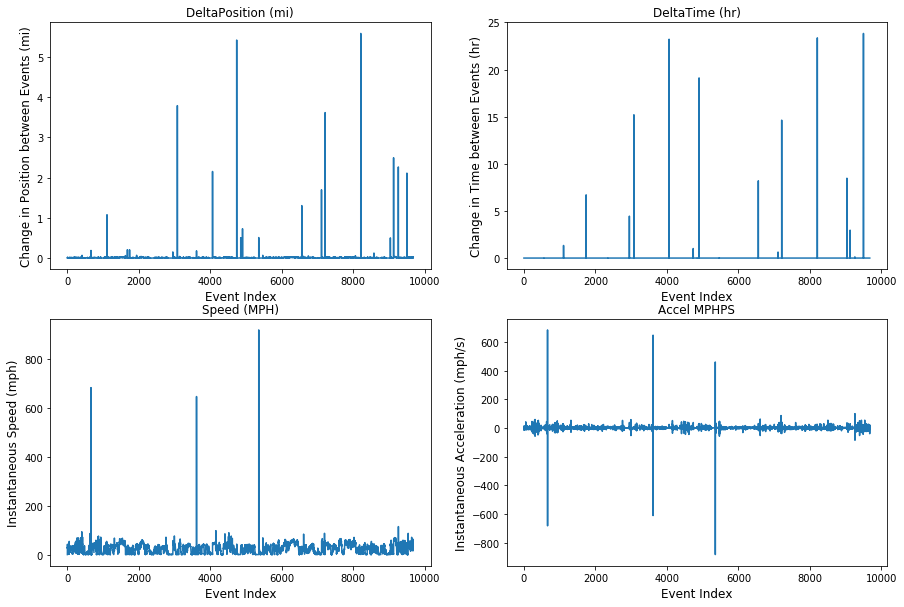
\includegraphics[width=1.\textwidth]{Images/Image3.png}
}

\frame{\frametitle{}
\begin{itemize}
\item
\end{itemize}
\centering
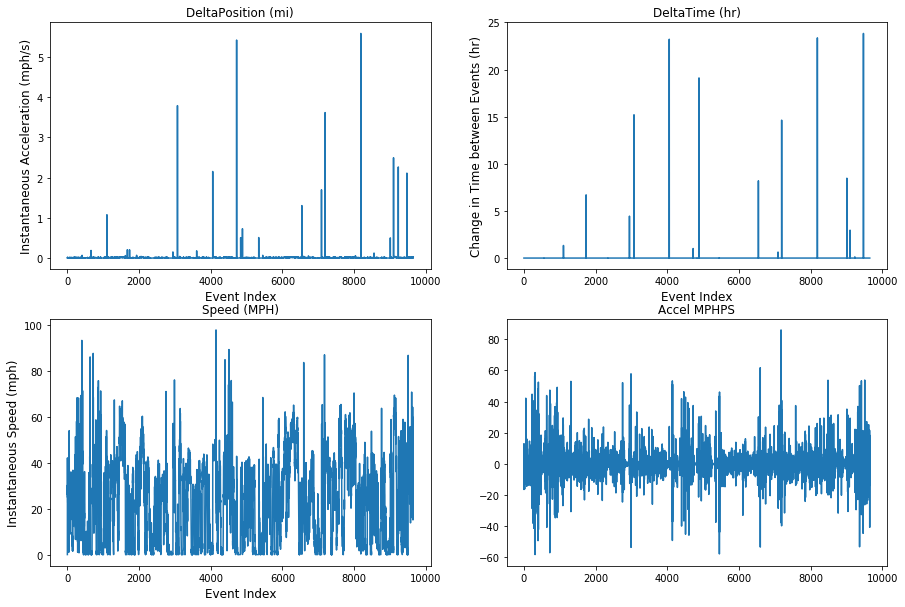
\includegraphics[width=1.\textwidth]{Images/Image4.png}
}

\frame{\frametitle{}
\begin{itemize}
\item
\end{itemize}
\centering
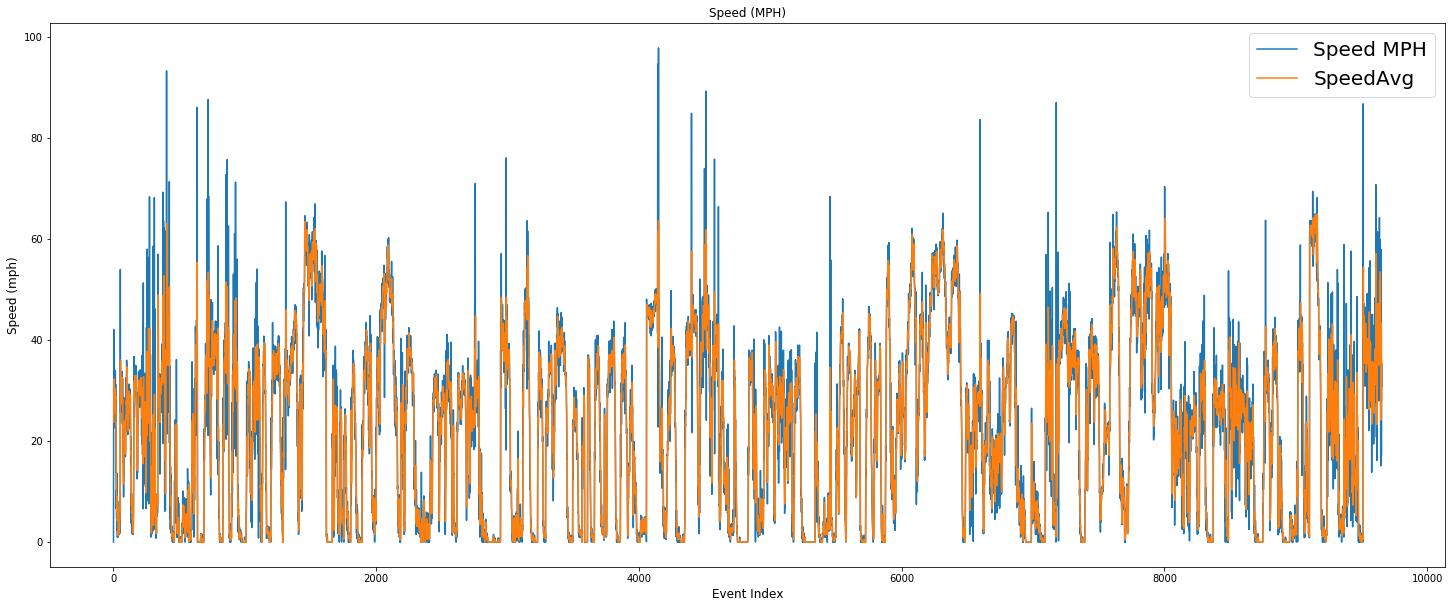
\includegraphics[width=1.\textwidth]{Images/Image5.png}
}

\frame{\frametitle{}
\begin{itemize}
\item
\end{itemize}
\centering
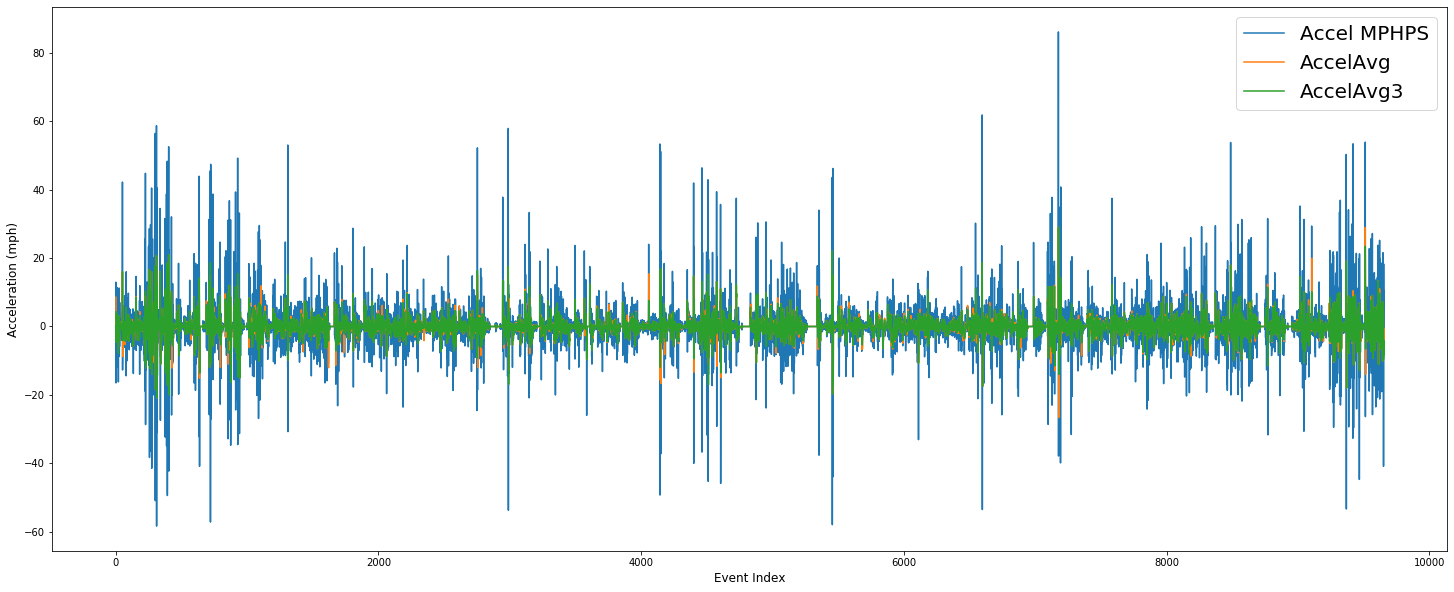
\includegraphics[width=1.\textwidth]{Images/Image6.png}
}

\frame{\frametitle{}
\begin{itemize}
\item
\end{itemize}
\centering
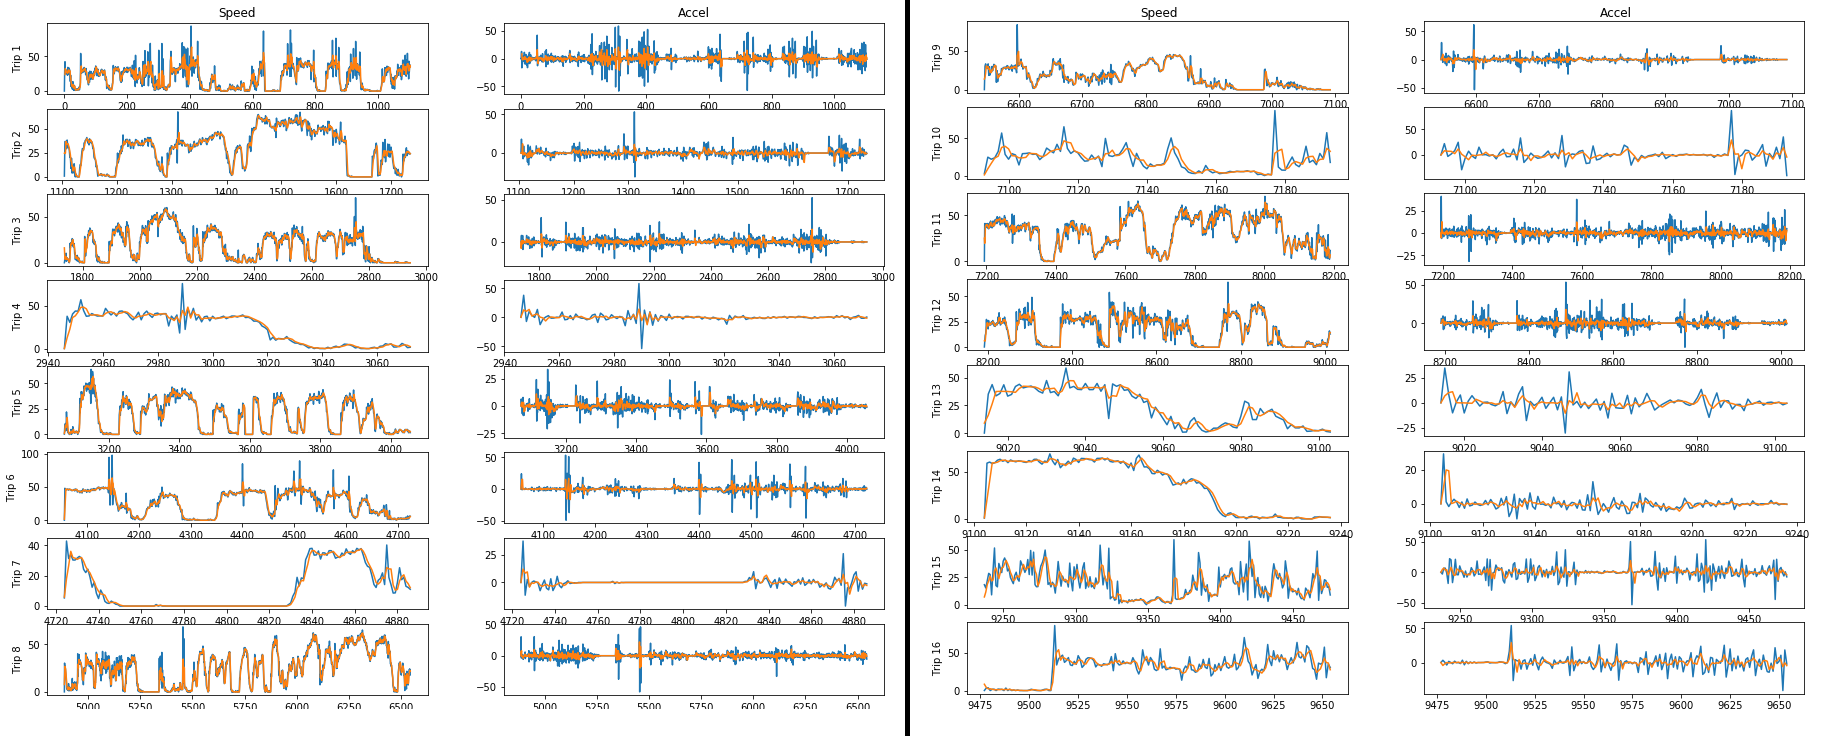
\includegraphics[width=1.\textwidth]{Images/Image7.png}
}

\frame{\frametitle{}
\begin{itemize}
\item
\end{itemize}
\centering
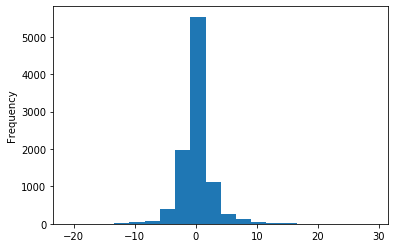
\includegraphics[width=0.5\textwidth]{Images/Image8.png}
}

\frame{\frametitle{}
\begin{itemize}
\item
\end{itemize}
\centering
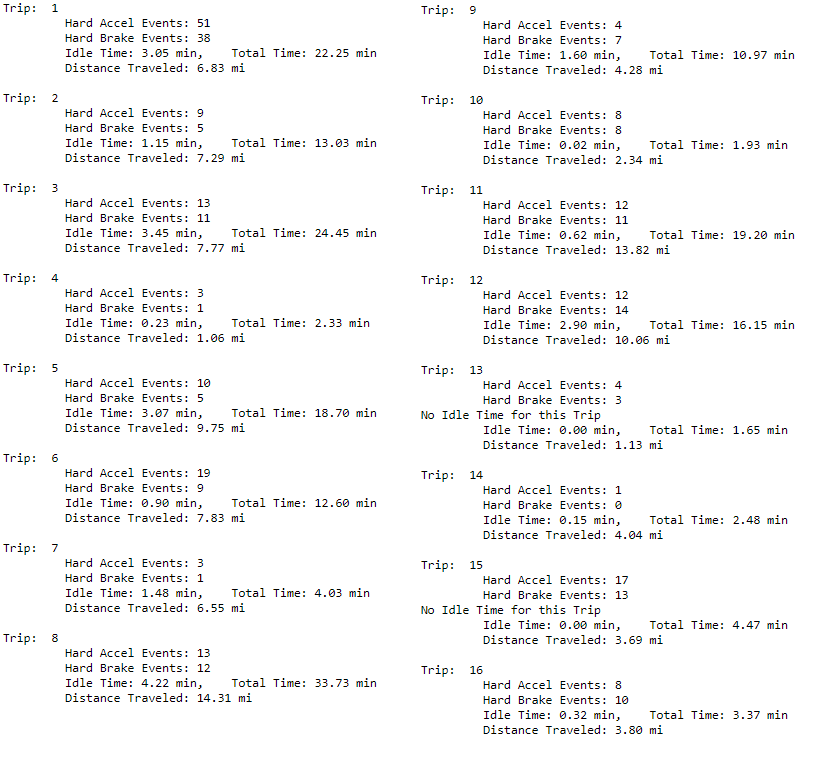
\includegraphics[width=0.7\textwidth]{Images/Image9.png}
}


\frame{\frametitle{FCNC: What are we looking for? $t\bar{t}\rightarrow W (\rightarrow l \nu) b+ q\gamma$}
\begin{itemize}
\item Final state topology
	\begin{itemize}
	\item One Neutrino, from W
	\item One Lepton, from W
	\item One B-jet, SM top
	\item \textbf{One Photon, FCNC Top}
	\item One Jet, FCNC Top
	\end{itemize}
\end{itemize}
}

\frame{\frametitle{Background Processes}
\begin{itemize}
\item Due to all of the processes at hadron colliders it is important to model similar event topologies well.
\item Major backgrounds include $t\bar{t}$, W+Jets, Z+Jets, + processes with an associated photon
\end{itemize}
%\centering
%\includegraphics[width=0.7\textwidth]{../../ThesisImages/backgrounds.png}
}

\frame{\frametitle{Monte Carlo Generation}
\begin{itemize}
\item All of our MC data is put through a showering algorithm for propagation from final decay states
\item Various showering algorithms are used at ATLAS - Pythia, Herwigg, etc.
\item All of these will add radiative photons
\item These events can be contained in other samples with explicit photons originating from the hard interaction
\item Need to remove these events or risk double counting events
\end{itemize}

}


%%%%%%%%%%%%%%%%%%%%%%%%%%%%%%%%%%%%%%%%%%%%%%%%%%%%%%%%%%%%%%%%%
\section{Part 2: Modeling}

\subsection{Object Preselection Cuts}

\frame{\frametitle{}
\begin{itemize}
\item
\end{itemize}
%\centering
%\includegraphics[width=0.7\textwidth]{../../ThesisImages/backgrounds.png}
}

\frame{\frametitle{Object Preselection}
\begin{itemize}
\item We preselect events with objects that look like our expected topology
\item Reminder that I require:
	\begin{itemize}
	\item Exactly one lepton (e or $\mu$) $\geq$ 28 GeV
	\item Exactly one Good photon $\geq$ 25GeV
	\item Missing Transverse Energy $\geq$ 30GeV
	\item $\geq 2$ Jets (at least one being b-tagged)
	\end{itemize}
\item All following plots will have signal scaled to $0.2\%$ of nonallhadronic $\sigma_{t\bar{t}}$, MC scaled to $36.07fb^{-1}$
\item Only electron channel shown.  Similar results for the muon channel are seen.
\end{itemize}
}


\subsection{Analysis}

\frame{\frametitle{Background Processes}
\begin{itemize}
\item Due to all of the processes at hadron colliders it is important to model similar event topologies well.
\item Major backgrounds include $t\bar{t}$, W+Jets, Z+Jets, + processes with an associated photon
\end{itemize}
%\centering
%\includegraphics[width=0.7\textwidth]{../../ThesisImages/backgrounds.png}
}
%%%%%%%%%%%%%%%%%%%%%%%%%%%%%%%%%%%%%%%%%%%%%%%%%%%%%%%%%%%%%%%%%%
\subsection{Model Building}

\frame{\frametitle{Background Processes}
\begin{itemize}
\item Due to all of the processes at hadron colliders it is important to model similar event topologies well.
\item Major backgrounds include $t\bar{t}$, W+Jets, Z+Jets, + processes with an associated photon
\end{itemize}
%\centering
%\includegraphics[width=0.7\textwidth]{../../ThesisImages/backgrounds.png}
}
\subsection{Data Set Enhancement}

\frame{\frametitle{Background Processes}
\begin{itemize}
\item Due to all of the processes at hadron colliders it is important to model similar event topologies well.
\item Major backgrounds include $t\bar{t}$, W+Jets, Z+Jets, + processes with an associated photon
\end{itemize}
%\centering
%\includegraphics[width=0.7\textwidth]{../../ThesisImages/backgrounds.png}
}

\section{Conclusion}
\frame{\frametitle{Conclusion, Outlook}
\begin{itemize}
\item Orthogonal validation/control regions are in development
\item Data grid run complete, need to incorporate into CR/VR plots
\item Next grid run will include a couple of looser regions for CR/VRs 
	\begin{itemize}
	\item 0 Photon Samples for Backgrounds with no Real Photons
	\item 0 BJet Samples - possibly for WJets region
	\end{itemize}
\item Top Group - Pushing for MVA, want to start investigations using these techniques 
\end{itemize}
}


%%%%%%%%%%%%%%%%%%%%%%%%%%%%%%%%%%%%%%%%%%%%%%%%%%%%%%%%%%%%%%%%
%%%%%%%%%%%%%%%%%%%%%%%%%%%%%%%%%%%%%%%%%%%%%%%%%%%%%%%%%%%%%%%% 	
\appendix
\section{Backup}
\frame{\frametitle{Backup}
}
\end{document}

%36.070
